%%%%%%%%%%%%%%%%%%%%%%%%%%%%%%%%%%%%%%%%%%%%%%%%%%%%%%%%%%%%%%%%%%%%%%%%%
%% Setup
%%%%%%%%%%%%%%%%%%%%%%%%%%%%%%%%%%%%%%%%%%%%%%%%%%%%%%%%%%%%%%%%%%%%%%%%%
%% set document class to article 
\documentclass[11pt]{article}

%% load packages 
\usepackage[left=1in,right=1in,top=1in,bottom=1in]{geometry} % set margins
\usepackage{amssymb, amsmath, amsfonts} % fonts, symbols, and formatting for equations 
\usepackage{rotating, pdflscape} % packages for rotating figures/tables/pages
\usepackage{setspace} % to set spacing (allows for double spacing) 
\usepackage[super,comma,compress]{natbib} % set citation format (superscript, separated by comma, condensed when possible)
\usepackage{color} % colored text
\usepackage{verbatim}
\usepackage{graphicx}
\usepackage[lofdepth,lotdepth]{subfig}
\usepackage{/home/lmalling/R/Sweave} % Sweave integration

%% specify page style
\setlength{\parindent}{0.0in}
\setlength{\parskip}{0.1in}

%% begin document 
\begin{document}
\bibliographystyle{plain}


%%%%%%%%%%%%%%%%%%%%%%%%%%%%%%%%%%%%%%%%%%%%%%%%%%%%%%%%%%%%%%%%%%%%%%%%%
%% Title Page
%%%%%%%%%%%%%%%%%%%%%%%%%%%%%%%%%%%%%%%%%%%%%%%%%%%%%%%%%%%%%%%%%%%%%%%%%
\title{CANTRANce Screening Aim}
\date{\today}
\author{Leslie Mallinger \\
		\small lmalling@fhcrc.org \\
		\small Etzioni Lab, Fred Hutchinson Cancer Research Center}
\maketitle


%%%%%%%%%%%%%%%%%%%%%%%%%%%%%%%%%%%%%%%%%%%%%%%%%%%%%%%%%%%%%%%%%%%%%%%%%%
%%% Background
%%%%%%%%%%%%%%%%%%%%%%%%%%%%%%%%%%%%%%%%%%%%%%%%%%%%%%%%%%%%%%%%%%%%%%%%%%
\section{Background}

The fundamental assumption underlying cancer screening is that early detection of a tumor will lead to correspondingly improved prognosis and disease-specific survival.
A key consequence of early detection is the reduction in the incidence of advanced cancers associated with the screening test.
Using user-specified inputs, CANTRANce will link comparative effectiveness study results on the reduction in the incidence of advanced tumors in the presence of a screening test into changes in disease-specific mortality and years of life saved under screening.

The general CANTRANce model for screening interventions is first discussed, then an example is provided using data {\color{red} with absolutely no grounding in reality whatsoever.}


%%%%%%%%%%%%%%%%%%%%%%%%%%%%%%%%%%%%%%%%%%%%%%%%%%%%%%%%%%%%%%%%%%%%%%%%%%
%%% Model Components
%%%%%%%%%%%%%%%%%%%%%%%%%%%%%%%%%%%%%%%%%%%%%%%%%%%%%%%%%%%%%%%%%%%%%%%%%%   
\section{Model Components}

%%%%%%%%%%%%%%%%%%%%%%%%%%%%%%%%%%%%
%%% Model Inputs
%%%%%%%%%%%%%%%%%%%%%%%%%%%%%%%%%%%%
\subsection{Model inputs}	

%%%%%%%%%%%%%%%%%
%%% Study data
%%%%%%%%%%%%%%%%%
\subsubsection{Comparative effectiveness study data}

The comparative effectiveness study data are entered into CANTRANce in one of two ways: 1) as individual-level data describing patient characteristics, or 2) as marginal distributions for patient characteristics. 
CANTRANce assumes a study design in which individual-level characteristics are linked with stage at clinical incidence, and a stage at incidence due to screening is assigned to each individual during the modeling process.

If individual-level data are available, the user will provide a data set in which the rows are individuals and columns contain data for each applicable patient characteristic.

If marginal distributions are to be used, the user may specify truncated normal distributions for continuous covariates and/or proportional distributions for categorical covariates. 

Regardless of entry method, required inputs are:
\begin{enumerate}
    \item \emph{male:} sex of individual
    \item \emph{age} or \emph{agegroup:} age of individual at time of clinical incidence. If \emph{age} is provided, users may specify desired age groups by which to perform analyses. If \emph{agegroup} is provided, single year ages are assigned to individuals by sampling from a uniform distribution within the given range.
    \item \emph{study\_year:} year of clinical incidence
    \item \emph{stage:} stage at time of \textbf{clinical} incidence
\end{enumerate}
Study data will often also include covariates that are expected to affect risk of disease-specific death or other-cause death.

%%%%%%%%%%%%%%%%%
%%% User options
%%%%%%%%%%%%%%%%%
\subsubsection{User specifications and assumptions}
Several choices must be made in how to use the comparative effectiveness study results to project mortality:
			
\begin{enumerate}
    \item \textbf{Population.} The user can choose to model the impact on the original study population, or on a population that is of a different size and/or has a different composition of covariates. 
				
    \item \textbf{Number of simulations.} Uncertainty due to modeling assumptions is computed by summarizing the results of many simulations. 
        Users may choose to run between 50 and 1,000 simulations.
				
    \item \textbf{Length of time to project.} CANTRANce will estimate mortality from the time of treatment through the length of time $t$ requested by the user.

    \item \textbf{Population-level stage distribution in presence of screening.} Stage at screened incidence is assigned during the modeling process based on clinical stage and the population-level stage distribution in the presence of screening. 

    In addition to the proportion of individuals in each stage in the presence of screening, the user must provide the order of the stages during natural progression of the disease, where 1 denotes the earliest, or least invasive stage of the disease, 2 denotes the next progression, etc.

    CANTRANce assigns stage at screened incidence using a cascade approach beginning with individuals in the most invasive stage of the disease at the time of clinical incidence.
    Some of these individuals will remain in the most invasive stage during screen-detection, and others will be shifted to an earlier stage.
    Thus, the appropriate number are sampled to remain in the highest stage, and the remainder are temporarily re-assigned to the second highest stage.
    Of those individuals in the second highest stage, a number are sampled to remain in that stage and the remainder are re-assigned to the next stage down in severity.
    The process continues for all remaining stages.
    In this way, some individuals undergo a ``stage shift'' due to screening, while the stage of others is unaffected by screening.
				
    \item \textbf{Time from clinical incidence to cause-specific death.} CANTRANce models time from clinical incidence to cause-specific death assuming an exponential process for the baseline cause-specific survival curve, with the option of applying modifications to the baseline curve for specified covariates.
				
    The user specifies the baseline cause-specific survival curve based on k-time survival, median survival, mean survival, or mortality rate in the absence of competing risks.
    Modified survival curves for up to three covariates may be specified either via hazard ratios or via survival statistics directly.
			
    \item \textbf{Time from clinical incidence to other-cause death.} For a typical population, time to other-cause death is approximated using US cohort lifetables matched to each individual by sex and year of birth. 
        If the study population is thought to be healthier or less healthy than the US population, the user can specify a hazard ratio to adjust the lifetable-based survival estimates. 
\end{enumerate}

%%%%%%%%%%%%%%%%%%%%%%%%%%%%%%%%%%%%
%%% Model Outputs
%%%%%%%%%%%%%%%%%%%%%%%%%%%%%%%%%%%%
\subsection{Model Outputs}

\begin{sidewaysfigure}
        \begin{center}
            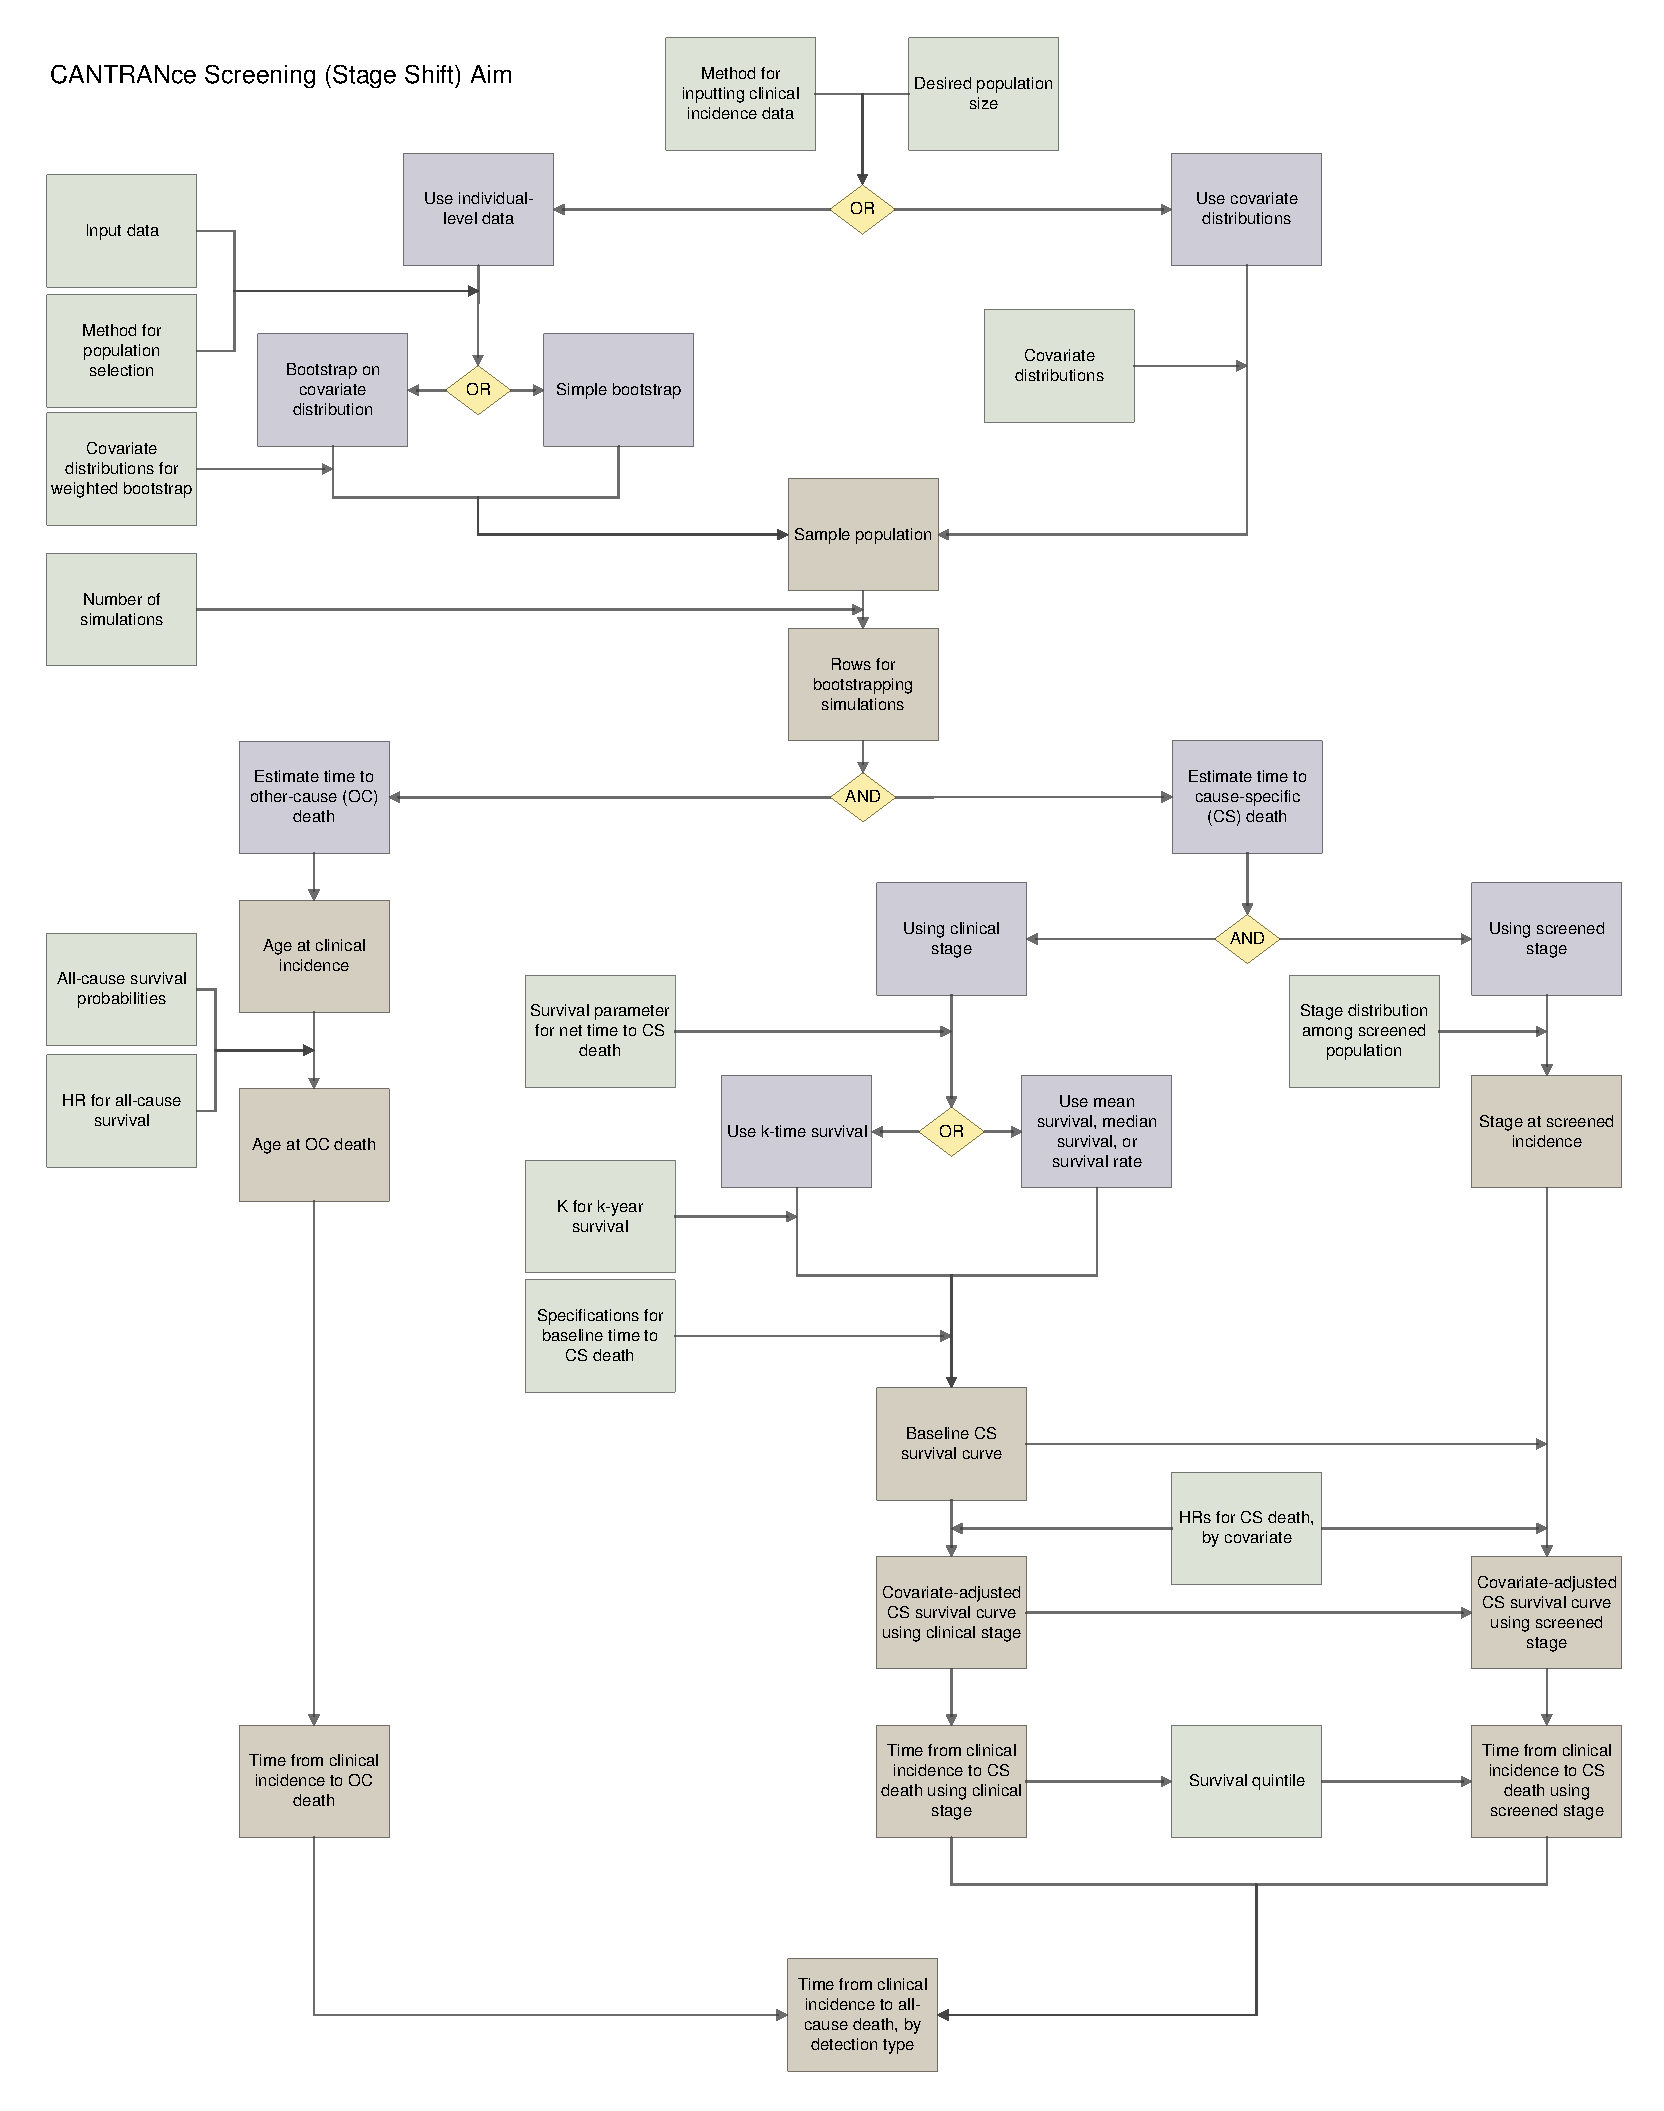
\includegraphics[width=0.65\textwidth]{../../documentation/flowchart_newstyle.pdf}
        \end{center}
        \caption{Flowchart representing the steps in the CANTRANce model for screening interventions. Green=user inputs. Purple=actions. Brown=intermediate results.}
        \label{fig:flowchart}
\end{sidewaysfigure}

Model inputs are processed according to the steps in Figure~\ref{fig:flowchart}. From treatment to the time $t$ specified by the user, CANTRANce will return:

\begin{enumerate}
	\item A table of mean, median, and $t$-time all-cause survival, and mean, median, and $t$-time net and crude disease-specific survival, presented as time from treatment to the outcome of interest. 
        While all-cause survival does not distinguish between disease-specific and other-cause death, net disease-specific survival censors other-cause deaths and represents the hypothetical scenario of survival from the disease in the absence of other-cause death, assuming that the two types of death are independent. 
        Crude disease-specific survival describes survival as it is observed; other-cause death is considered a competing event that precludes death from the disease, so other-cause deaths are not considered at risk after their death. 
        It follows from this definition of at-risk time that crude disease-specific survival is always higher than net disease-specific survival; in the latter, the censoring of other-cause death implies the possibility of disease-specific death at future times \cite{kim_cumulative_2007}.
			
    \item Survival curves for all-cause survival, net disease-specific survival, and crude disease-specific survival.
			
    \item A table of person-years saved by the screening intervention among the study popuation during the period from enrollment to time $t$.

    \item A table of cause-specific mortality statistics describing the mortality trends observed in the simulated population, stratified by covariate and mode of detection when applicable. This table allows the user to verify that simulated times to event are consistent with the times to event specified as user inputs.

    \item A table of statistics describing the time by which cause-specific death was delayed, stratified by stage at clinical diagnosis.
\end{enumerate}

%%%%%%%%%%%%%%%%%%%%%%%%%%%%%%%%%%%%
%%% Model Validation
%%%%%%%%%%%%%%%%%%%%%%%%%%%%%%%%%%%%
\subsection{Model Validation}
{\color{red} We should brainstorm ways to validate the model.}


%%%%%%%%%%%%%%%%%%%%%%%%%%%%%%%%%%%%%%%%%%%%%%%%%%%%%%%%%%%%%%%%%%%%%%%%%%
%%% Example 
%%%%%%%%%%%%%%%%%%%%%%%%%%%%%%%%%%%%%%%%%%%%%%%%%%%%%%%%%%%%%%%%%%%%%%%%%% 
\section{Example: {\color{red}Random Inputs}}

The user inputs used in this example were just picked to illustrate the functionality of the screening aim, and don't represent true data.

%%%%%%%%%%%%%%%%%%%%%%%%%%%%%%%%%%%%
%%% Model Inputs
%%%%%%%%%%%%%%%%%%%%%%%%%%%%%%%%%%%%
\subsection{Model Inputs}


%%%%%%%%%%%%%%%%%
%%% Study data
%%%%%%%%%%%%%%%%%
\subsubsection{Comparative effectiveness study data}

Study participants consisted of $100$ men assigned characteristics at clinical incidence according to the distributions in Tables~\ref{tab:age}-\ref{tab:tx}. 
The date of clinical incidence was assumed to be $2000$ for all participants.

Individual ages were generated from a truncated normal with specifications shown in Table~\ref{tab:age}, then categorized into groups with ages 50-64, 65-69, and 70-74.


% latex table generated in R 3.0.1 by xtable 1.7-1 package
% Wed Jul  3 13:23:28 2013
\begin{table}[!ht]
\centering
\begin{tabular}{ccccc}
  \hline
Variable & Mean & SD & Min & Max \\ 
  \hline
age & 65 & 7 & 55 & 74 \\ 
   \hline
\end{tabular}
\caption{Population characteristics for age (years)} 
\label{tab:age}
\end{table}

Tables~\ref{tab:sg} and \ref{tab:tx} give the proportion of individuals assigned to each clinical stage, grade, and treatment group.
Note that a joint distributions was specified for stage and grade, as these are believed to covary, whereas treatment was assumed to be independent of other characteristics.


% latex table generated in R 3.0.1 by xtable 1.7-1 package
% Wed Jul  3 13:23:28 2013
\begin{table}[!ht]
\centering
\begin{tabular}{ccc}
  \hline
Clinical Stage & Grade & Proportion \\ 
  \hline
Localized & Low & 0.20 \\ 
  Localized & High & 0.10 \\ 
  Regional & Low & 0.15 \\ 
  Regional & High & 0.15 \\ 
  Distant & Low & 0.05 \\ 
  Distant & High & 0.35 \\ 
   \hline
\end{tabular}
\caption{Proportions of individuals in each clinical stage and grade group} 
\label{tab:sg}
\end{table}
% latex table generated in R 3.0.1 by xtable 1.7-1 package
% Wed Jul  3 13:23:28 2013
\begin{table}[!ht]
\centering
\begin{tabular}{cc}
  \hline
Treatment & Proportion \\ 
  \hline
Prostatectomy & 0.2 \\ 
  Radiation & 0.4 \\ 
  Other & 0.4 \\ 
   \hline
\end{tabular}
\caption{Proportions of individuals in each treatment group} 
\label{tab:tx}
\end{table}
%%%%%%%%%%%%%%%%%
%%% User options
%%%%%%%%%%%%%%%%%	
\subsubsection{User specifications and assumptions}

\begin{enumerate}
    \item \textbf{Population.} The model population for each simulation consisted of $100$ individuals with clinical incidence in $2000$.

    \item \textbf{Number of simulations.} $50$ 

    \item \textbf{Length of time to project.} Mortality was projected for $50$ years from the time of treatment.

    \item \textbf{Population-level stage distribution in presence of screening.} The proportion of individuals presenting in each stage in the presence of screening is shown in Table ~\ref{tab:scrdist}, as is the order of stage progression. 


% latex table generated in R 3.0.1 by xtable 1.7-1 package
% Wed Jul  3 13:23:28 2013
\begin{table}[!ht]
\centering
\begin{tabular}{ccc}
  \hline
Order & Screened Stage & Proportion \\ 
  \hline
  1 & Localized & 0.50 \\ 
    2 & Regional & 0.30 \\ 
    3 & Distant & 0.20 \\ 
   \hline
\end{tabular}
\caption{Proportions of individuals in each stage in presence of screening} 
\label{tab:scrdist}
\end{table}
    Recall that the stage distribution among individuals at clinical incidence was 30\% in localized, 30\% in regional, and 40\% in distant stage.

    The stage shift was implemented as follows: of the 40\% of individuals who were clinically incident in distant stage, half (20\% of the total population) were sampled to stay in distant stage for their screened incidence, and the remaining half (20\% of the total population) were temporarily shifted to regional stage, bringing the population total in regional stage to 30\% + 20\% = 50\%.
    Then, of the 50\% of individuals in regional stage, 2/3 (30\% of the total population) were sampled to stay in regional stage for their screened incidence, and the remaining 1/3 (20\% of the total population) were shifted to local stage.
    This brought the total in local stage to 30\% + 20\% = 50\%, as desired.

    Note that individuals with distant clinical stage could be assigned to any of the three screened stages, but individuals with local clinical stage stayed in local stage upon screening.

    FIXME To do: Add a ``cure'' state to shift into.

    \item \textbf{Time from clinical incidence to cause-specific death.} For the baseline survival curve, 5-year cause-specific survival was 0.68.
        Survival statistics were specified separately by clinical stage and primary treatment (Table~\ref{tab:morthrs}).
        For this example, stage-specific survival was specified in terms of 5-year cause-specific survival, which CANTRANce used to calculate survival rates and corresponding hazard ratios to modify baseline survival.
        Treatment-specific survival was already provided by the user in terms of hazard ratios.
        The hazard ratio for each individual was calculated as the product of hazard ratios for each group to which he belonged.


% latex table generated in R 3.0.1 by xtable 1.7-1 package
% Wed Jul  3 13:23:28 2013
\begin{table}[!ht]
\centering
\begin{tabular}{llc}
  \hline
Risk & Group & HR \\ 
  \hline
Clinical Stage & Localized & 0.39 \\ 
   & Regional & 1.00 \\ 
   & Distant & 2.95 \\ 
  Treatment & Prostatectomy & 0.65 \\ 
   & Radiation & 0.90 \\ 
   & Other & 1.00 \\ 
   \hline
\end{tabular}
\caption{Hazard ratio for cause-specific death, by clinical stage and treatment} 
\label{tab:morthrs}
\end{table}
    \item \textbf{Time from intervention to other-cause death.} Time to other-cause death was approximated using unadjusted US cohort lifetables matched by sex and year of birth.

\end{enumerate}

%%%%%%%%%%%%%%%%%%%%%%%%%%%%%%%%%%%%
%%% Model Outputs
%%%%%%%%%%%%%%%%%%%%%%%%%%%%%%%%%%%%
\subsection{Model Outputs}


% latex table generated in R 3.0.1 by xtable 1.7-1 package
% Wed Jul  3 13:23:28 2013
\begin{table}[!ht]
\centering
\begin{tabular}{lccc}
  \hline
Measure & Mode & Mean.Survival & Median.Survival \\ 
  \hline
All-Cause Survival & Clinical & 8.240 (6.630-10.16) & 5.940 (4.140-7.900) \\ 
  All-Cause Survival & Screened & 9.820 (8.100-11.61) & 7.810 (5.910-10.57) \\ 
  Net Survival & Clinical & 17.95 (13.07-22.81) & 8.230 (5.860-11.63) \\ 
  Net Survival & Screened & 24.56 (19.18-30.28) & 13.41 (8.830-19.31) \\ 
  Crude Survival & Clinical &  & 10.39 (6.820-17.62) \\ 
  Crude Survival & Screened &  & 18.14 (11.79-29.22) \\ 
   \hline
\end{tabular}
\caption{Mean and  median survival for three survival metrics, by mode of detection. Parentheses give 2.5\% and 97.5\% quantiles across simulations. Survival times are measured from time of clinical incidence.} 
\label{tab:mmsurv}
\end{table}
% latex table generated in R 3.0.1 by xtable 1.7-1 package
% Wed Jul  3 13:23:28 2013
\begin{table}[!ht]
\centering
\begin{tabular}{lcccc}
  \hline
Measure & Mode & Five.Year & Ten.Year & Fifty.Year \\ 
  \hline
All-Cause Survival & Clinical & 0.539 (0.429-0.645) & 0.308 (0.222-0.421) & 0.000100 (0.000100-0.000100) \\ 
  All-Cause Survival & Screened & 0.621 (0.536-0.704) & 0.403 (0.292-0.509) & 0.000500 (0.000500-0.000500) \\ 
  Net Survival & Clinical & 0.625 (0.513-0.722) & 0.434 (0.357-0.530) & 0.0849 (0.0405-0.135) \\ 
  Net Survival & Screened & 0.721 (0.639-0.789) & 0.563 (0.459-0.647) & 0.139 (0.0704-0.203) \\ 
  Crude Survival & Clinical & 0.645 (0.539-0.740) & 0.491 (0.417-0.594) & 0.383 (0.304-0.468) \\ 
  Crude Survival & Screened & 0.738 (0.654-0.805) & 0.612 (0.522-0.703) & 0.495 (0.414-0.578) \\ 
   \hline
\end{tabular}
\caption{5-year, 10-year, and 50-year survival for three survival metrics, by mode of detection. Parentheses give 2.5\% and 97.5\% quantiles across simulations. Survival times are measured from time of clinical incidence.} 
\label{tab:ksurv}
\end{table}

\begin{figure}[!ht]
    \centering
    \includegraphics[width=\textwidth]{../output/survival_results.pdf}
    \caption{All-cause, crude cause-specific, and net cause-specific survival curves, by mode of detection. Survival times are measured from time of clinical incidence.}
    \label{fig:surv}
\end{figure}
	
Table~\ref{tab:mmsurv} gives the number of years for mean and median all-cause survival and net and crude cause-specific survival from the time of clinical incidence. 5-year, 10-year, and 50-year survival proportions are provided in Table~\ref{tab:ksurv}.
Blank cells indicate that the metric could not be calculated given available information.
Corresponding survival curves are shown in Figure~\ref{fig:surv}. 

During the 50 years following treatment, 158 (90 to 236) person-years were saved by screening.

Table~\ref{tab:csm} shows five-year cause-specific survival by risk group and mode of diagnosis, as specified by the user and observed in the simulated population. Observed values are close to those designated in the inputs, and if only one covariate is chosen (not shown), the values are nearly identical.

Table~\ref{tab:delay} shows the delay in cause-specific mortality due to the stage shift induced by screening, by stage at clinical incidence. As expected, screening has no impact on individuals with localized clinical stage, because they remained in localized stage even under screen-detection.


% latex table generated in R 3.0.1 by xtable 1.7-1 package
% Wed Jul  3 13:23:28 2013
\begin{table}[!ht]
\centering
\begin{tabular}{lllcc}
  \hline
Risk & Group & Mode & User Input & Observed \\ 
  \hline
All Individuals & - & Clinical &  & 0.684 (0.616-0.769) \\ 
   & - & Screened &  & 0.771 (0.715-0.830) \\ 
  Stage & Localized & - & 0.860 & 0.882 (0.829-0.928) \\ 
   & Regional & - & 0.680 & 0.713 (0.633-0.790) \\ 
   & Distant & - & 0.320 & 0.370 (0.210-0.504) \\ 
  Treatment & Prostatectomy & - & 0.778 & 0.781 (0.661-0.876) \\ 
   & Radiation & - & 0.707 & 0.722 (0.623-0.838) \\ 
   & Other & - & 0.680 & 0.703 (0.589-0.810) \\ 
   \hline
\end{tabular}
\caption{5-year cause-specific survival specified by the user and observed in the simulated population, by risk group and mode of diagnosis.} 
\label{tab:csm}
\end{table}

% latex table generated in R 3.0.1 by xtable 1.7-1 package
% Wed Jul  3 13:23:28 2013
\begin{table}[!ht]
\centering
\begin{tabular}{lc}
  \hline
Clinical Stage & Estimate \\ 
  \hline
Localized & 0.000 (0.000-0.000) \\ 
  Regional & 9.227 (3.270-15.20) \\ 
  Distant & 9.573 (4.441-16.01) \\ 
   \hline
\end{tabular}
\caption{Delay in cause-specific mortality due to screening-induced stage shift, by stage at clinical incidence.} 
\label{tab:delay}
\end{table}

%%%%%%%%%%%%%%%%%%%%%%%%%%%%%%%%%%%%%%%%%%%%%%%%%%%%%%%%%%%%%%%%%%%%%%%%%
%% Bibliography
%%%%%%%%%%%%%%%%%%%%%%%%%%%%%%%%%%%%%%%%%%%%%%%%%%%%%%%%%%%%%%%%%%%%%%%%%
\bibliography{bibfile.bib}

\end{document}

